
%% Beispiel-Präsentation mit LaTeX Beamer im KIT-Design
%% entsprechend den Gestaltungsrichtlinien vom Februar 2025
%%
%% Siehe https://sdq.kastel.kit.edu/wiki/Dokumentvorlagen

%% Beispiel-Präsentation
\documentclass[]{sdqbeamer} 
 
%% Gruppenlogo, muss im Verezeichnis logos/ liegen
%% falls kein Gruppenlogo gewünscht, bitte \grouplogo{} aufrufen
\grouplogo{} 

%% Gruppenname und Breite (Standard: 89 mm)
\groupname{Software Design and Quality}
%\groupnamewidth{89mm}

% Beginn der Präsentation

%Information to be included in the title page:
\title{Combining Memory-Efficient Parallel SAT Solving and Distributed Clause Sharing}
\subtitle{Master Thesis}
\author{Ruben Götz}

\date[11.\,9.\,2025]{11. September 2025}

% Literatur 
 
\usepackage[citestyle=authoryear,bibstyle=numeric,hyperref,backend=biber]{biblatex}
%\addbibresource{presentation.bib}
\bibhang1em

\usepackage{lipsum}
\usepackage{booktabs}
\usepackage{subcaption}


% 20-25 Minuten ist die Norm für einen Mastervortrag. 
% Eine kurze Einleitung für Menschen, die SAT Solving 
% schonmal gehört haben, ganz kurz der relevante 
% Stand der Technik, deine Contributions als Hauptteil 
% und die wichtigsten Ergebnisse aus der Evaluation 
% (dem kannst du denke ich viel Gewicht geben, weil 
% das dann auch den Schwerpunkt deiner MA spiegelt). 


%\begin{minipage}{0.5\textwidth}
%...
%\end{minipage}%
%\begin{minipage}{0.5\textwidth}
%...
%\end{minipage}%

\begin{document}

%Titelseite
\begin{frame}[title white vertical, picture=images/palladio_bauplan]
	\titlepage
\end{frame}

%%%%%%%%%%%%%%%%%%%555

\section{Introduction}
\begin{frame}{Introduction}
    \begin{block}{SAT Solving}
        Given a Boolean formula (usually in CNF):
        \begin{itemize}
            \item Decide whether Formula is SAT
            \item Give assignment if Formula is SAT
        \end{itemize}
    \end{block}

    \begin{exampleblock}{$F = (a \lor b) \land (\lnot a \lor c \lor d)$}
        Is SAT for examplary assignment $a = false, b = true, c = false, d = false$
    \end{exampleblock}
\end{frame}

\begin{frame}{Introduction}
    \begin{block}{Usecases}
        \begin{itemize}
            \item Hardware and Software verification
            \item Automated Planning
            \item Scheduling
            \item Cryptoanalysis
            \item (explainable) AI
            \item Theorem Proving
            \item $\cdots$
        \end{itemize}
    \end{block}
\end{frame}

%%%%%%%%%%%%%%%%%%%%%%%%%%

\section{State of the Art}
\begin{frame}{State of the Art}
    \begin{block}{Serial SAT solvers}
        \begin{itemize}
            \item Mostly based on CDCL algorithm
            \item i.e. learns conflict clauses
        \end{itemize}
    \end{block}

    \begin{block}{Parallel SAT solvers}
        \begin{itemize}
            \item Search Space Partitioning: Divide problem into disjoint subspaces
            \item Portfolio Solvers: Run multiple diverse serial solvers in parallel
            \begin{itemize}
                \item Increase efficiency by sharing clauses
                \item Distributed SAT solving is on the rise
                \item Annual SAT competition includes cloud track since 2020
                % \item MallobSat
            \end{itemize}
        \end{itemize}
    \end{block}
\end{frame}

\begin{frame}{State of the Art}
    \begin{block}{Memory-Efficient SAT solving}
        \begin{itemize}
            \item Most research focuses on runtime
            \item Running independent solver engines comes with inherent memory redundancy
            \item[$\Rightarrow$] Gimsatul utilizes shared clauses in Memory
        \end{itemize}
    \end{block}

    \begin{block}{Contributions}
        \begin{itemize}
            \item Integrate Gimsatul into MallobSat to combine memory efficiency with scalability
            \item Implement \textit{search only} approach [\href{https://satres.kikit.kit.edu/papers/2025-sat-streamlining-pre.pdf}{Schreiber et al.~2025}]
            \item Evaluate approach experimentally
        \end{itemize}
    \end{block}
\end{frame}

% Ich hab Mallob jetzt als 2023 anegeben, aber das Paper aus 2024 verlinkt
\begin{frame}{How MallobSat Works [\href{https://www.jair.org/index.php/jair/article/download/15827/27072}{Schreiber\&Sanders.~2023}]}
    \center
    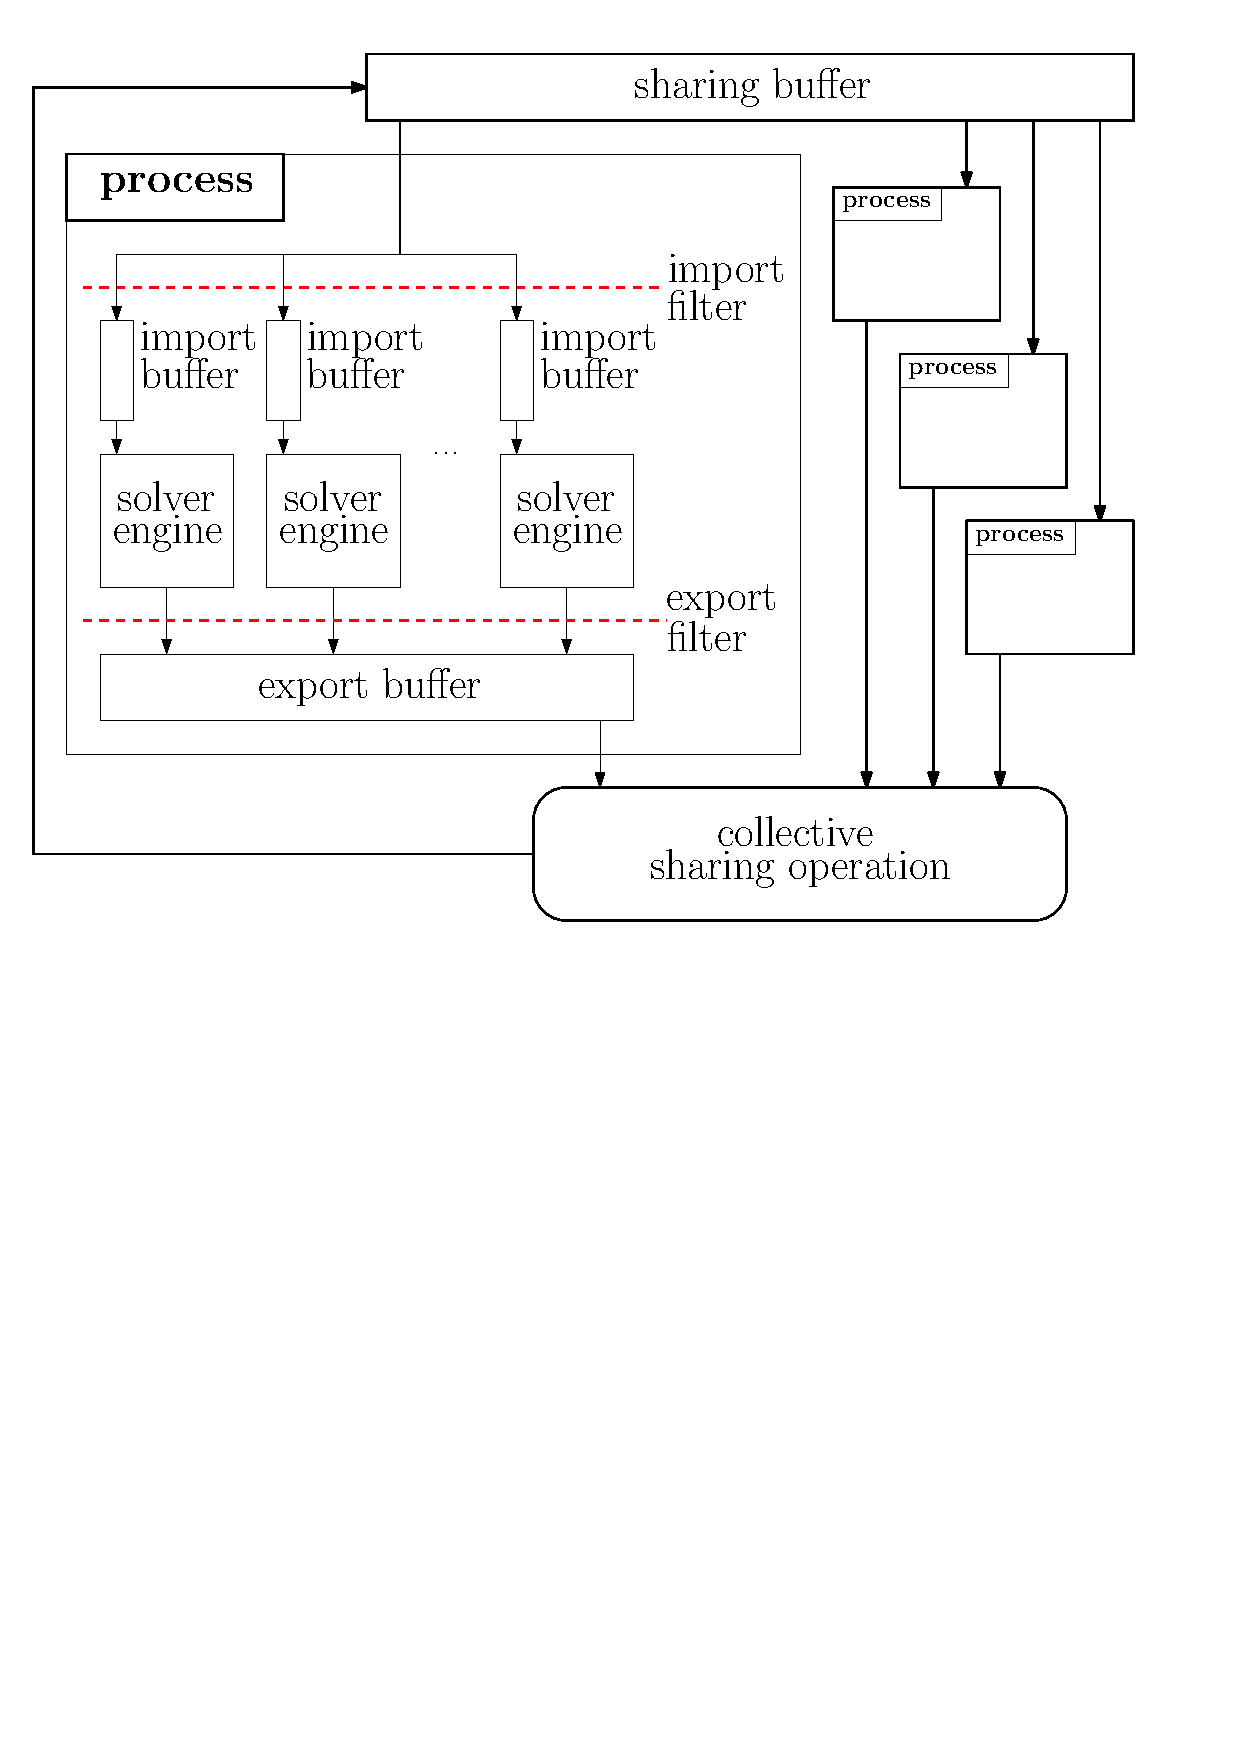
\includegraphics[scale=.8]{figures/mallob_architecture.pdf}
\end{frame}

\begin{frame}{How Gimsatul Works [\href{https://arxiv.org/pdf/2207.13577}{Fleury\&Biere.~2022}]}
    \center
    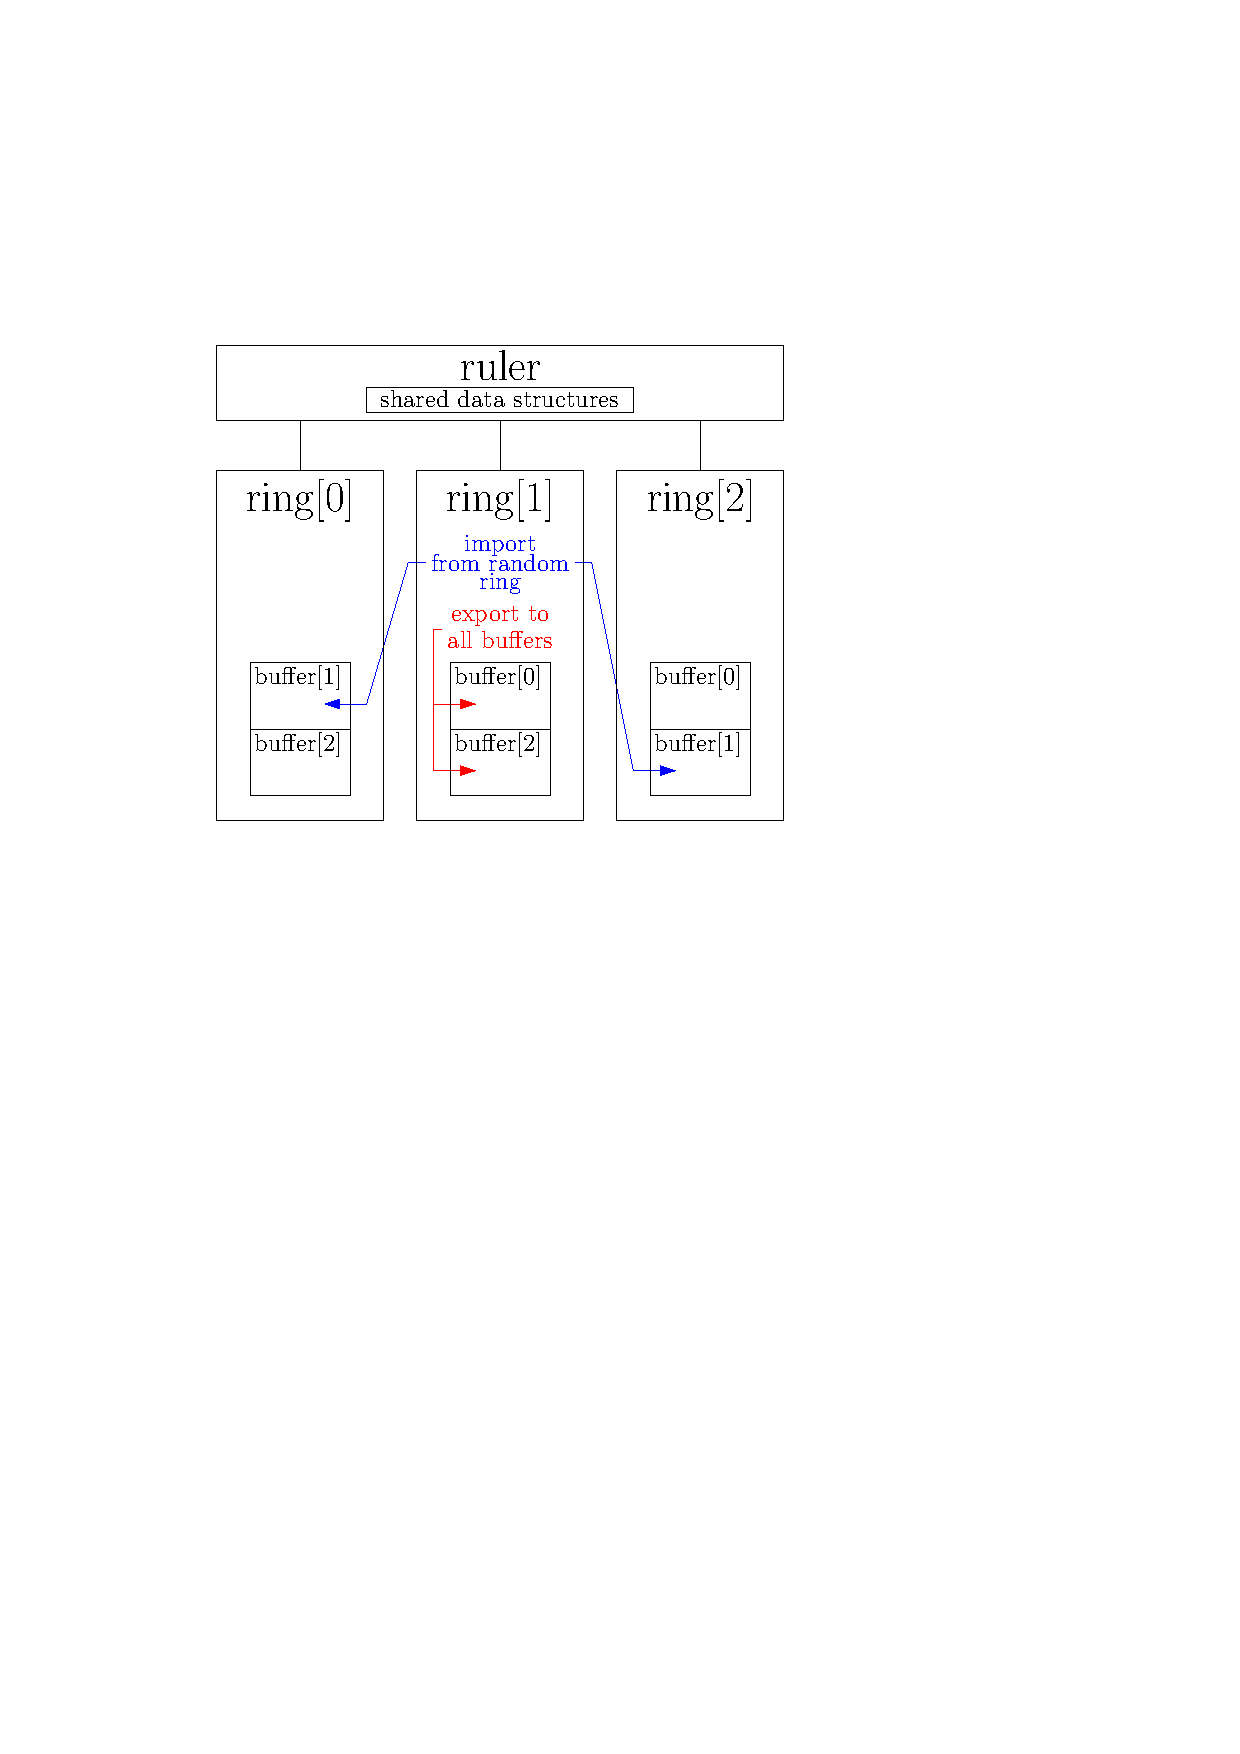
\includegraphics[scale=1.5]{figures/gimsatul_architecture.pdf}
\end{frame}

%%%%%%%%%%%%%%%%%%%%%%%%%%%%%%55

\section{Our Architecture}
\begin{frame}{Our Architecture}
    \center
    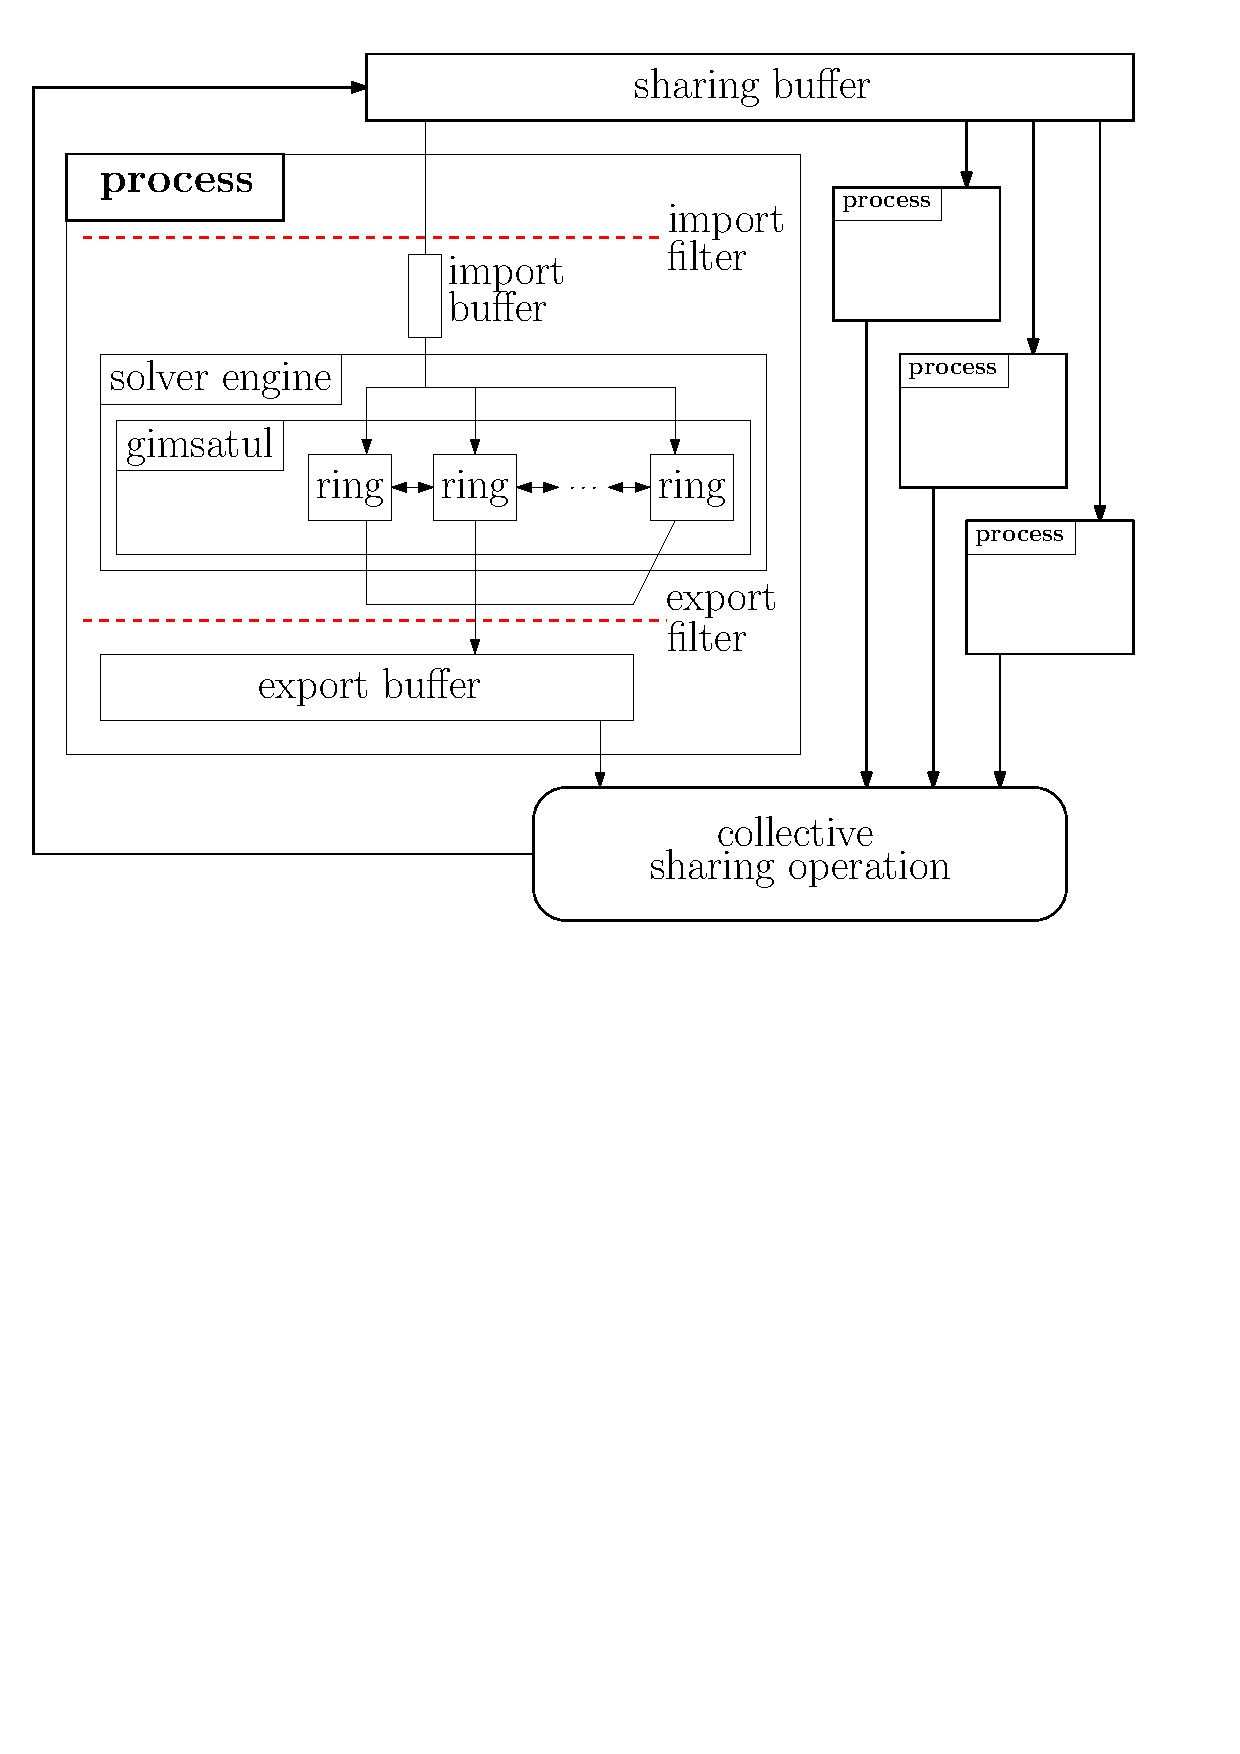
\includegraphics[scale=.8]{figures/architecture.pdf}
\end{frame}

\begin{frame}{Our Architecture}
    \begin{block}{Creating the Solver Engine}
        If Gimsatul is part of portfolio:
        \begin{itemize}
            \item Accumulate all $t'$ threads, that are defined to be Gimsatul
            \item Run Gimsatul with $t'$ threads
            \item MallobSat process runs with $t$ threads and $t - t' + 1$ solver engines
            \item extend Gimsatul's diversification
        \end{itemize}
    \end{block}
\end{frame}

\begin{frame}{Our Architecture}
    \begin{block}{Clause Export}
        \begin{itemize}
            \item All rings export externally if they export internally
            \item MallobSat's clause sharing mechanisms elegantly handles...
            \begin{itemize}
                \item[...] Clause filtering
                \item[...] Avoiding redundant clause sharing
            \end{itemize}
        \end{itemize}
    \end{block}

    \begin{block}{Clause Import}
        \begin{itemize}
            \item All rings import independently
            \item If there are conflicts, importing is skipped
            \item A ring imports at most as many clauses as there are rings in its Gimsatul instance
        \end{itemize}
    \end{block}
\end{frame}

\begin{frame}{Our Architecture}
    \begin{block}{Diversification}
        Added \textit{sparse random variable phases} on top of Gimsatuls native diversification:
        \begin{itemize}
            \item Flip phases of random variables
            \item $p = 1 / e$ for $e$ engines in total
            \item implemented as $p = 1 / (t' * p)$ for $t'$ rings and $p$ processes
        \end{itemize}
    \end{block}
\end{frame}

\begin{frame}{Our Architecture}
    \begin{minipage}{0.45\textwidth}
        \center
        \begin{block}{Search Only}
            \begin{itemize}
                \item Proposed by Schreiber, Rigi-Luperti \& Biere in 2025
                \item Deactivate pre- and inprocessing
                \item Run single dedicated preprocessing job in the beginning
                \item Replace jobs with preprocessed formula over time
            \end{itemize}
        \end{block}
    \end{minipage}%
    \hfill
    \begin{minipage}{0.45\textwidth}
        \center
        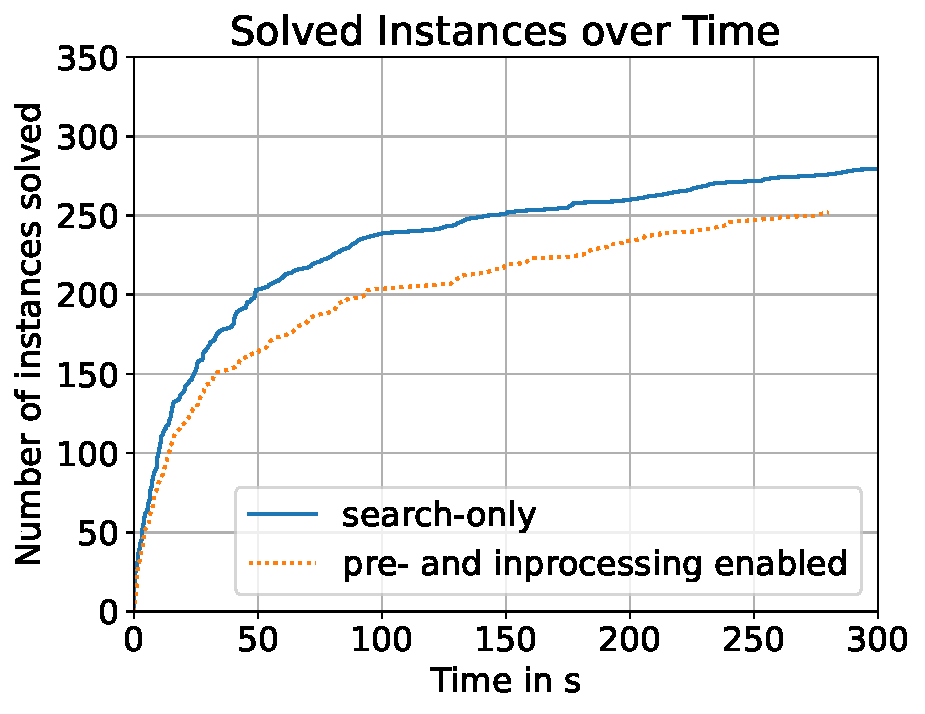
\includegraphics[scale=.8]{plots/config_compare/search_only_compare.pdf}
    \end{minipage}%

\end{frame}

%%%%%%%%%%%%%%%%%%%%%%%%%%%%%%%%%%

\section{Experimental Evaluation}
\begin{frame}{Benchmarks \& Configuration}
    \begin{block}{Benchmarks}
        Benchmarks were provided by Iser and Jabs in 
        their Global Benchmark Database. Specifically, 
        we used the track \textit{main\_2024}.
    \end{block}

    \begin{block}{Configuration}
        \begin{itemize}
            \item Experiments done on SuperMUC
            \begin{itemize}
                \item 1 node contains 48 cores (96 Hardware threads)
                \item used up to 16 nodes (768 cores)
            \end{itemize}
            \item 1 Gimsatul instance per node
            \item 48 threads per node
            \item Search Only approach
        \end{itemize}
    \end{block}
\end{frame}

\begin{frame}{Runtime}
    \center
    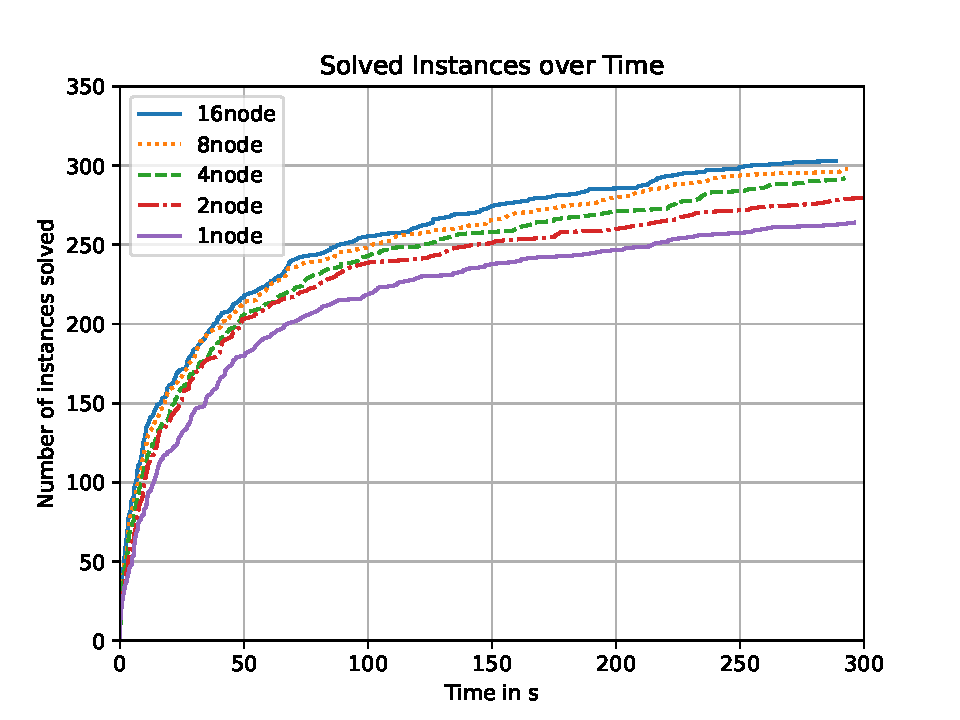
\includegraphics[scale=1]{plots/cumulative_runtime/scalability_gim.pdf}
\end{frame}

\begin{frame}{Speedups}
    \begin{minipage}{.45\textwidth}
        \noindent
        \center
        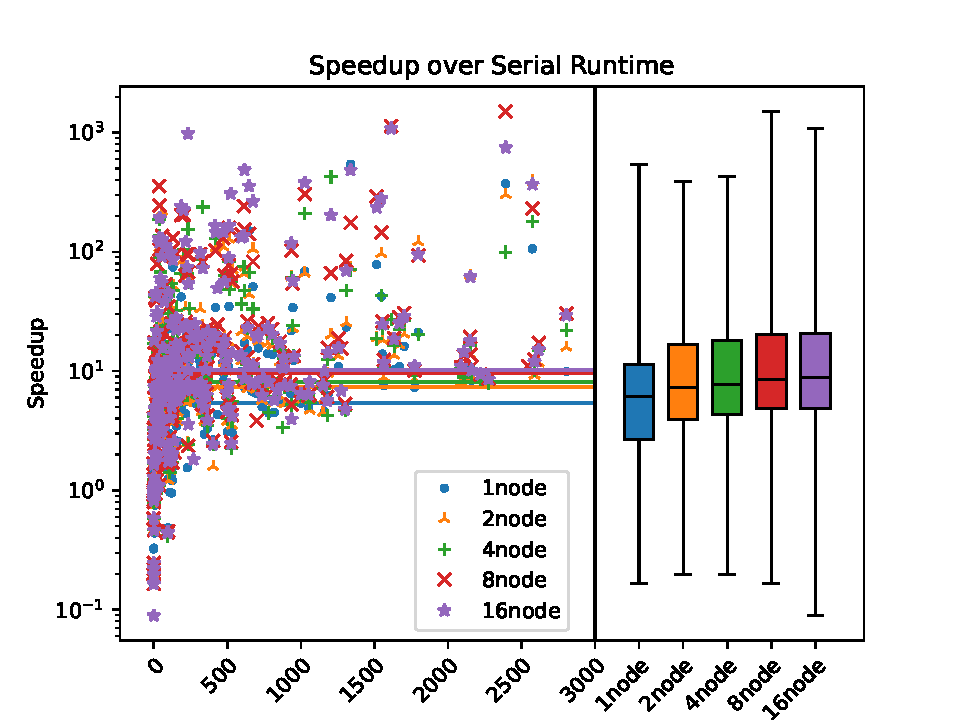
\includegraphics[scale=.6]{plots/speedups_gim.pdf}
    \end{minipage}
    \hfill
    \begin{minipage}{.45\textwidth}
        \noindent
        \center
        \begin{table}[!h]
            \begin{tabular}{ cccc }
                \toprule
                \#cores & gm Speedup\\
                \midrule
                48 & 5.357\\
                96 & 7.384\\
                192 & 8.146\\
                384 & 9.720\\
                768 & 10.260\\
              \bottomrule
            \end{tabular}
        %\caption{Geometric mean speedups for number of cores.}
    \end{table}
    \end{minipage}
\end{frame}

\begin{frame}{Comparison to MallobSat}
    \begin{minipage}{0.45\textwidth}
        \center
        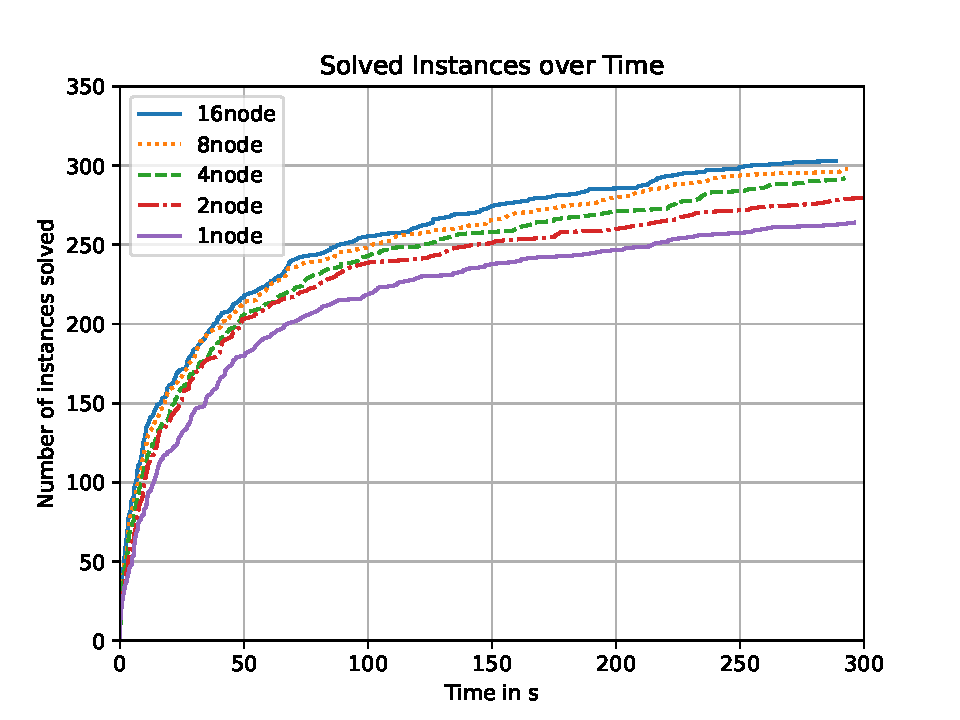
\includegraphics[scale=.8]{plots/cumulative_runtime/scalability_gim.pdf}\\
        Scalability of our approach
    \end{minipage}
    \hfill
    \begin{minipage}{0.45\textwidth}
        \center
        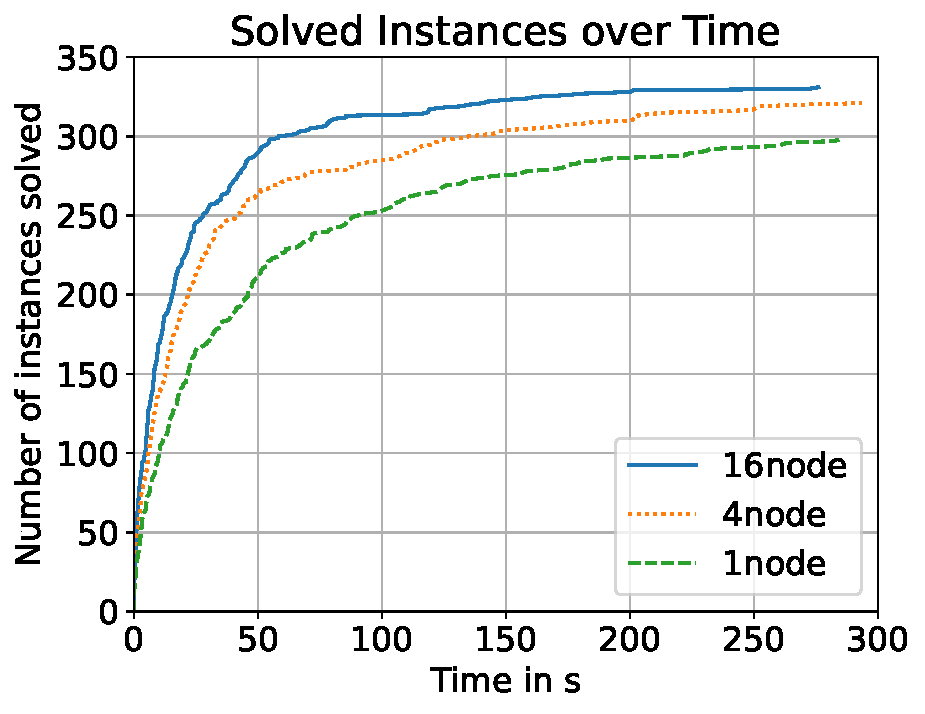
\includegraphics[scale=.8]{plots/cumulative_runtime/scalability_kis.pdf}\\
        Scalability of MallobSat%' default configuration
    \end{minipage}
\end{frame}

\begin{frame}{Comparison to MallobSat}
    \center
    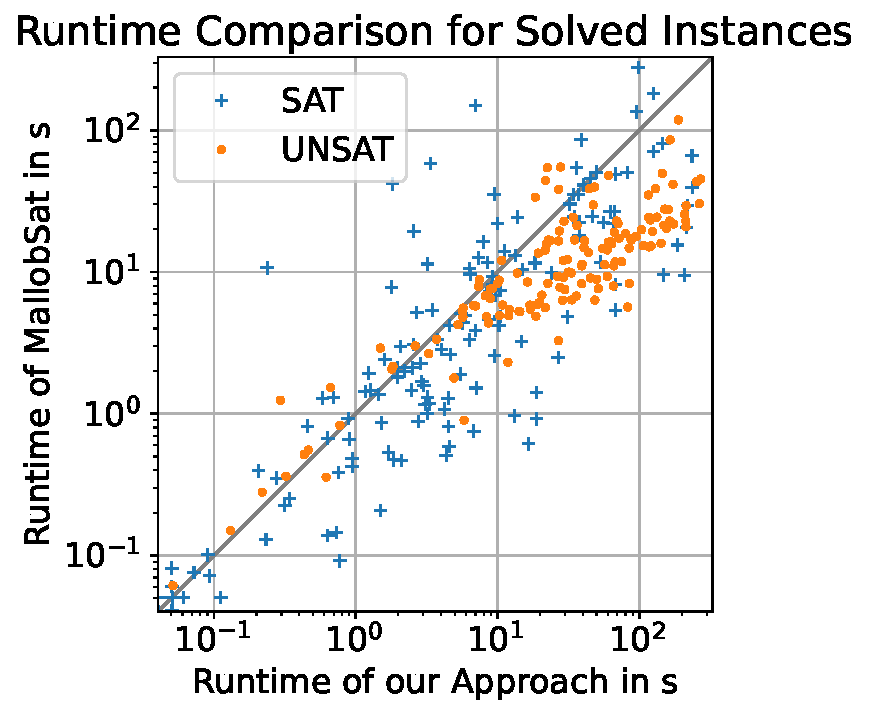
\includegraphics[scale=.8]{plots/square_runtime_compare/square_runtime_16node.pdf}\\
    Runtime Comparison between MallobSat and our approach, using 16 nodes.
\end{frame}

\begin{frame}{}
    \center
    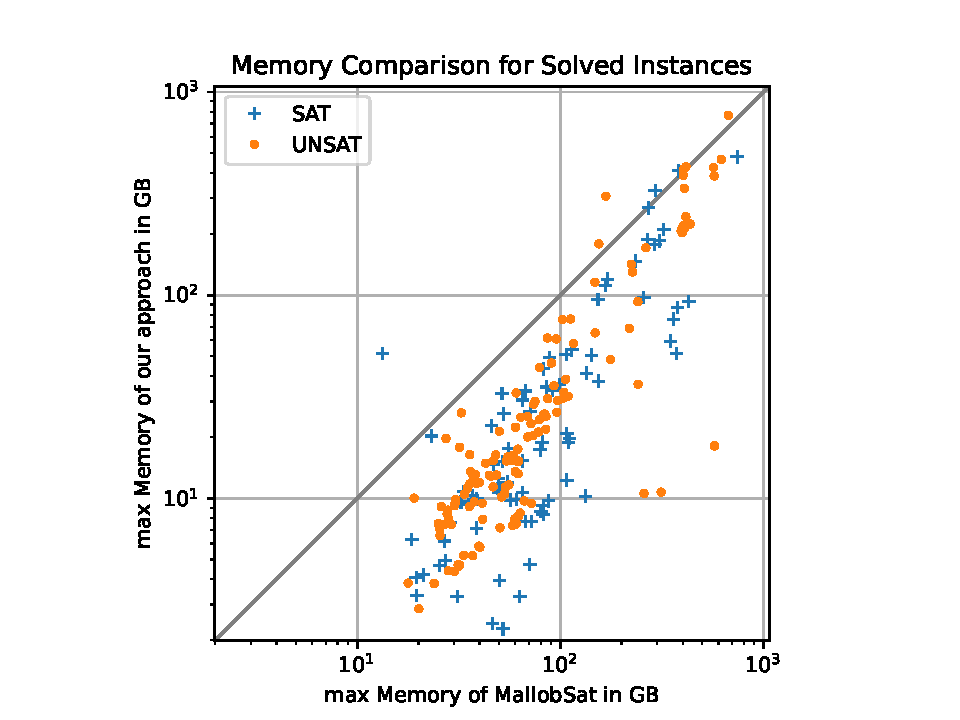
\includegraphics[scale=.8]{plots/square_mem_compare/square_mem_16node.pdf}\\
    Memory Comparison between MallobSat and our approach, using 16 nodes.
\end{frame}

\begin{frame}{Comparison to MallobSat}
    \center
    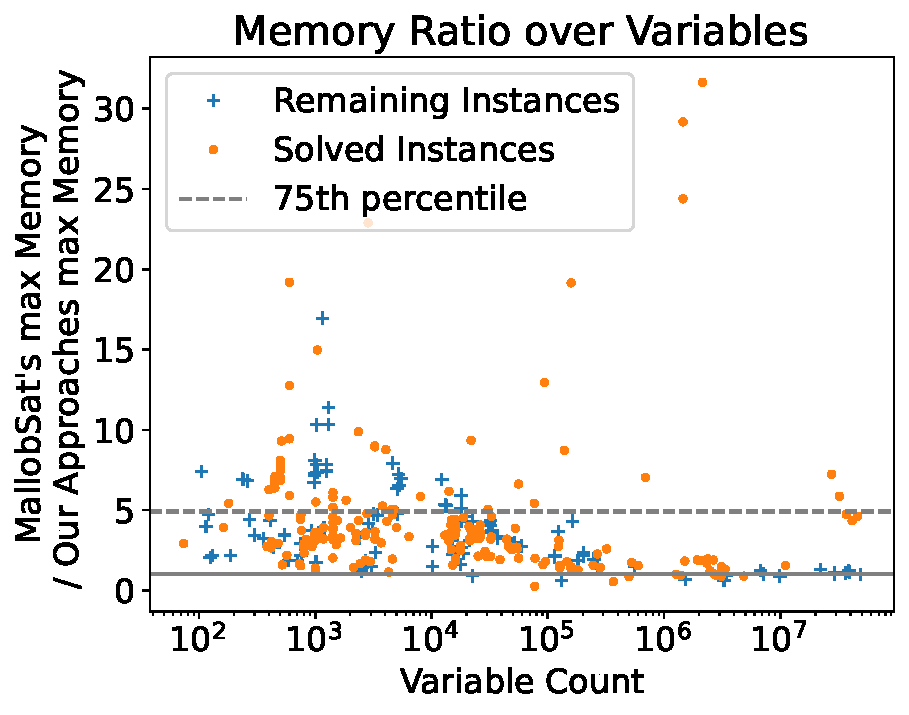
\includegraphics[scale=.8]{plots/16node_compare/mem_ratio_over_vars.pdf}\\
    Memory ratios between MallobSat and our approach, using 16 nodes. Each data point corresponds to a benchmark instance.
\end{frame}

\begin{frame}{Comparison to MallobSat}
    \center
    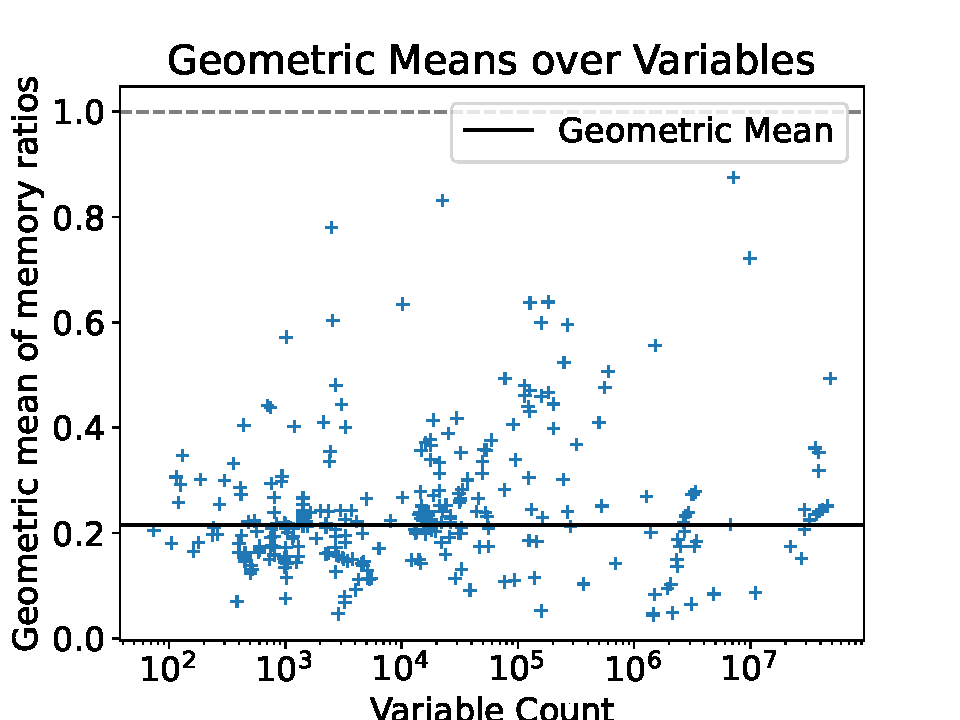
\includegraphics[scale=.8]{plots/16node_compare/mem_gm_over_vars.pdf}\\
    Geometric means for memory ratios between MallobSat and our approach per second, using 16 nodes. Each data point corresponds to a benchmark instance.
\end{frame}

\begin{frame}{Comparison to MallobSat}
    \center
    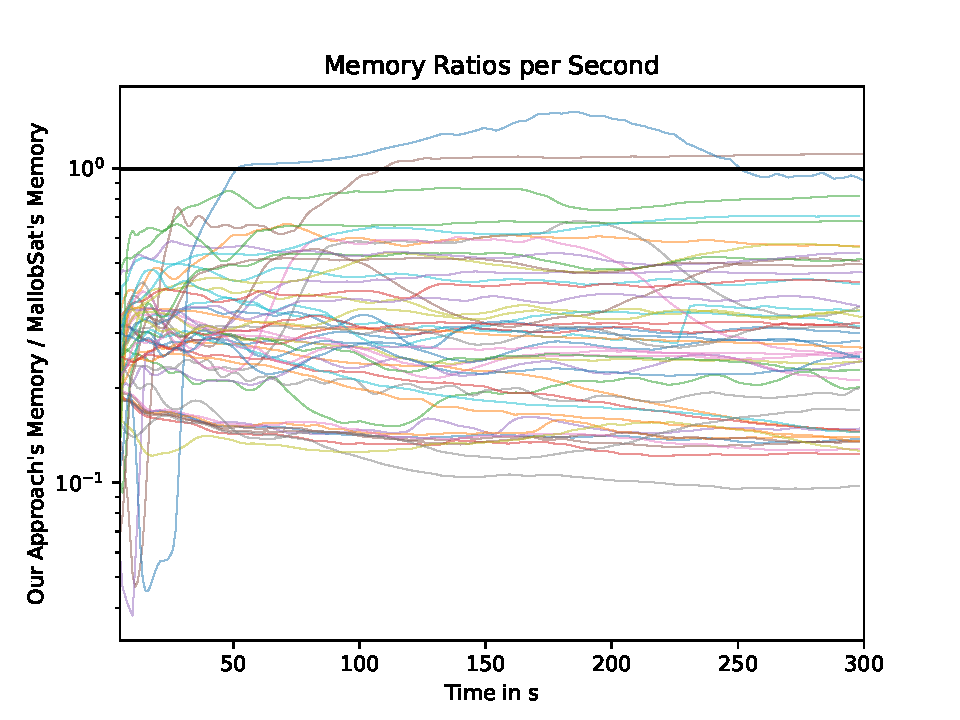
\includegraphics[scale=.8]{plots/16node_compare/mem_ratio_per_second.pdf}\\
    Memory ratios per second for all instances that reached the timeout of $300\,$s (both with MallobSat and our approach), using 16 nodes. % The lines were smoothed, using a sliding window of size five seconds and calculating its geometric mean.
\end{frame}

\begin{frame}{Comparison to MallobSat}
    \center
    \begin{table}[scale=.75]
        \center
        \begin{tabular}{ ccccc }
          \toprule
          \multicolumn{1}{c}{} & \multicolumn{2}{c}{Overall Used Memory} & \multicolumn{2}{c}{Normalized}\\
          \#cores & Our Approach & MallobSat & Our Approach & MallobSat \\
          \midrule
          48  & 0.149 & 0.089 & 7.140 & 4.256\\
          96  & 0.076 & -     & 7.306 & -\\
          192 & 0.039 & 0.026 & 7.583 & 5.036\\
          384 & 0.020 & -     & 7.780 & -\\
          768 & 0.010 & 0.006 & 7.766 & 4.924\\
          \bottomrule
        \end{tabular}
    \end{table}
    \vfill
    Solved instances per GB of overall used memory in the middle and the same values normalized by the number of cores on the right.
\end{frame}

\begin{frame}{Interesting Tidbits}
    \centering
    \begin{table}[!h]
        \center
        \begin{tabular}{ lcccccc }
            \toprule
            family	&	\#	&	1node	&	2node	&	4node	&	8node	&	16node\\
            \midrule
            heule-folkman	&	11	&	0.425	&	-	&	0.416	&	0.449	&	0.444\\
            cryptography-simon	&	10	&	0.221	&	0.234	&	0.227	&	0.2	&	0.18\\
            miter	&	47	&	1.705	&	1.835	&	1.997	&	2.25	&	2.013\\
            \vdots &&&&&&\\
            % random-circuits	&	15	&	2.598	&	3.095	&	3.527	&	3.849	&	3.839\\
            % planning	&	6	&	2.567	&	3.977	&	4.168	&	4.623	&	4.835\\
            % software-verification	&	15	&	2.564	&	5.073	&	4.248	&	4.57	&	4.71\\
            % tseitin-formulas	&	8	&	4.442	&	4.567	&	5.177	&	5.275	&	5.49\\
            % hardware-verification	&	5	&	4.621	&	5.369	&	5.556	&	6.036	&	6.161\\
            % scheduling	&	50	&	5.333	&	6.434	&	7.944	&	8.384	&	8.799\\
            % heule-nol	&	11	&	5.988	&	11.793	&	7.786	&	10.231	&	12.876\\
            % cryptography-ascon	&	6	&	7.396	&	8.273	&	10.115	&	8.709	&	14.008\\
            % maxsat-optimum	&	13	&	7.419	&	7.32	&	12.362	&	13.762	&	14.899\\
            % quantum-kochen-specker	&	10	&	9.356	&	11.237	&	11.186	&	11.137	&	11.005\\
            % cryptography	&	7	&	6.32	&	16.922	&	9.289	&	21.402	&	23.632\\
            % hamiltonian	&	40	&	8.968	&	14.409	&	19.398	&	23.315	&	26.351\\
            % argumentation	&	21	&	13.01	&	16.268	&	18.577	&	21.941	&	20.716\\
            independent-set	&	15	&	16.442	&	18.038	&	20.981	&	27.173	&	25.9\\
            minimum-disagreement-parity	&	17	&	40.311	&	22.119	&	24.766	&	46.884	&	58.316\\
            rbsat	&	5	&	47.606	&	64.654	&	76.039	&	186.204	&	221.286\\
            \bottomrule
        \end{tabular}
    \end{table}
    \vfill
    Geometric mean speedups per family and setup, for families comprising at least 5 instances and a calculatable speedup.
\end{frame}

%%%%%%%%%%%%%%%%%%%%%%%%%%%%%%%%%%%%

\section{Conclusion}
\begin{frame}{Conclusion}
    \begin{block}{Summary}
        \begin{itemize}
            \item Integrated Gimsatul into MallobSat as solver engine
            \item Evaluated approach
        \end{itemize}
    \end{block}

    \begin{block}{Conclusion}
        \begin{itemize}
            \item Succeeded in stated goal to increase memory-efficiency
            \item Elevator Pitch: \textbf{4x less memory} than default configuration
            \begin{itemize}
                \item gm of gm of Memory Ratios between MallobSat's default configuration and our approach is 0.25
            \end{itemize}
            \item Runtime tradeoff
        \end{itemize}
    \end{block}
\end{frame}

\end{document}
